\begin{frame}
\frametitle{Scena: Demo}

\begin{columns}

\column{.5\textwidth}

\begin{figure}[ht]
    \centering
    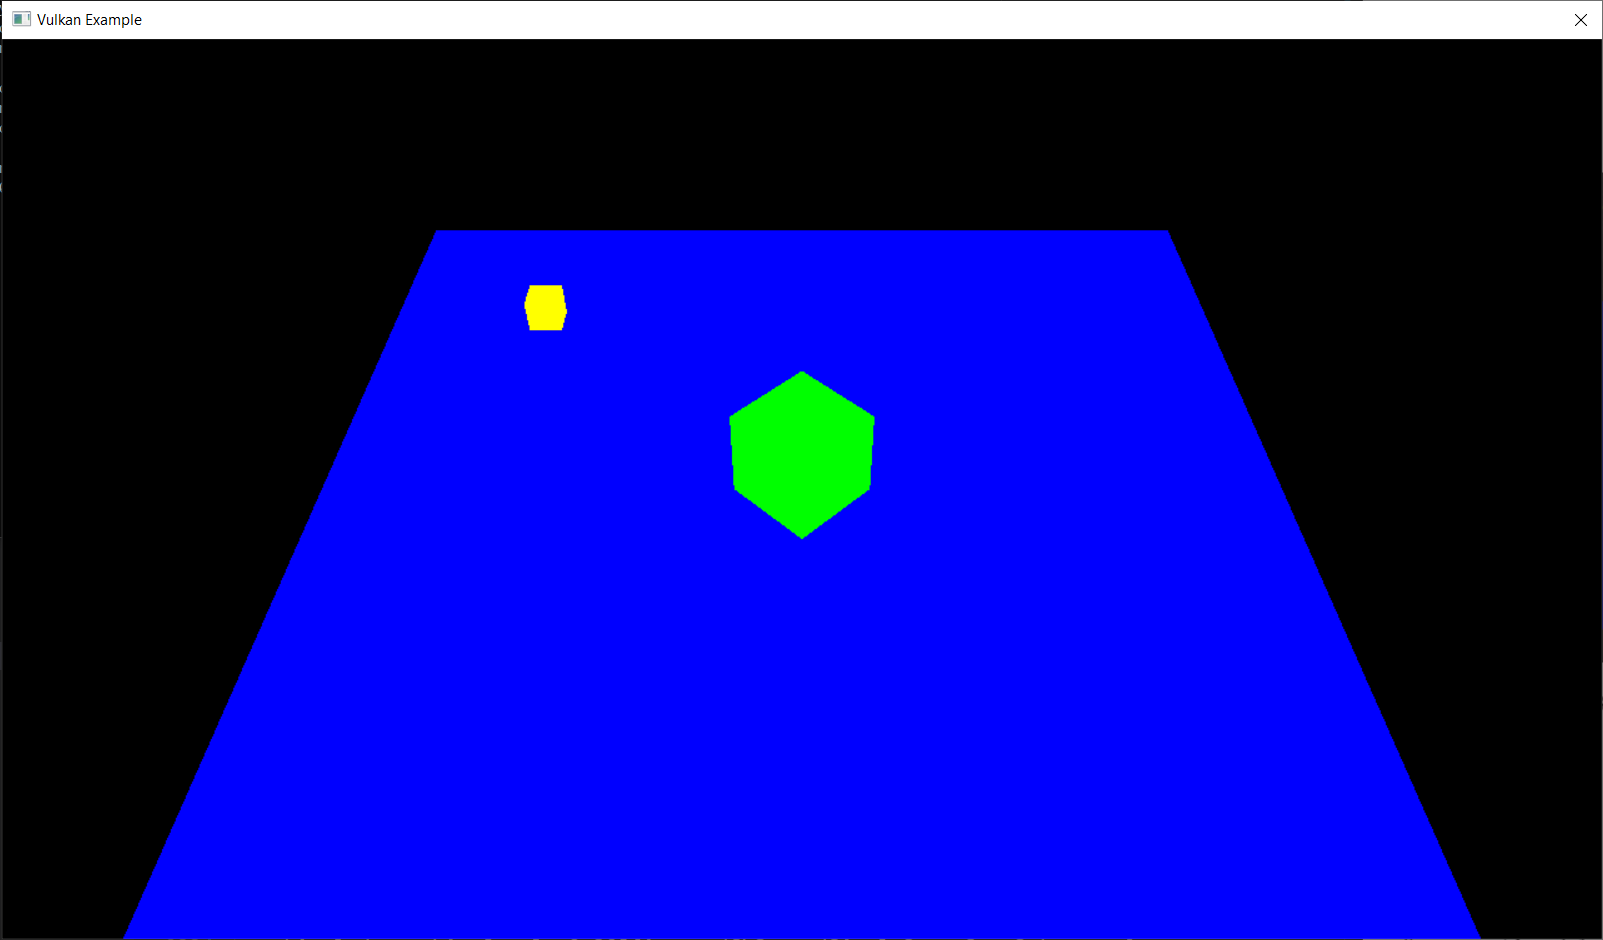
\includegraphics[scale=0.14]{images/SlidesScene/SimpleScene.png}
\end{figure}

\column{.5\textwidth}

\begin{figure}[ht]
    \centering
    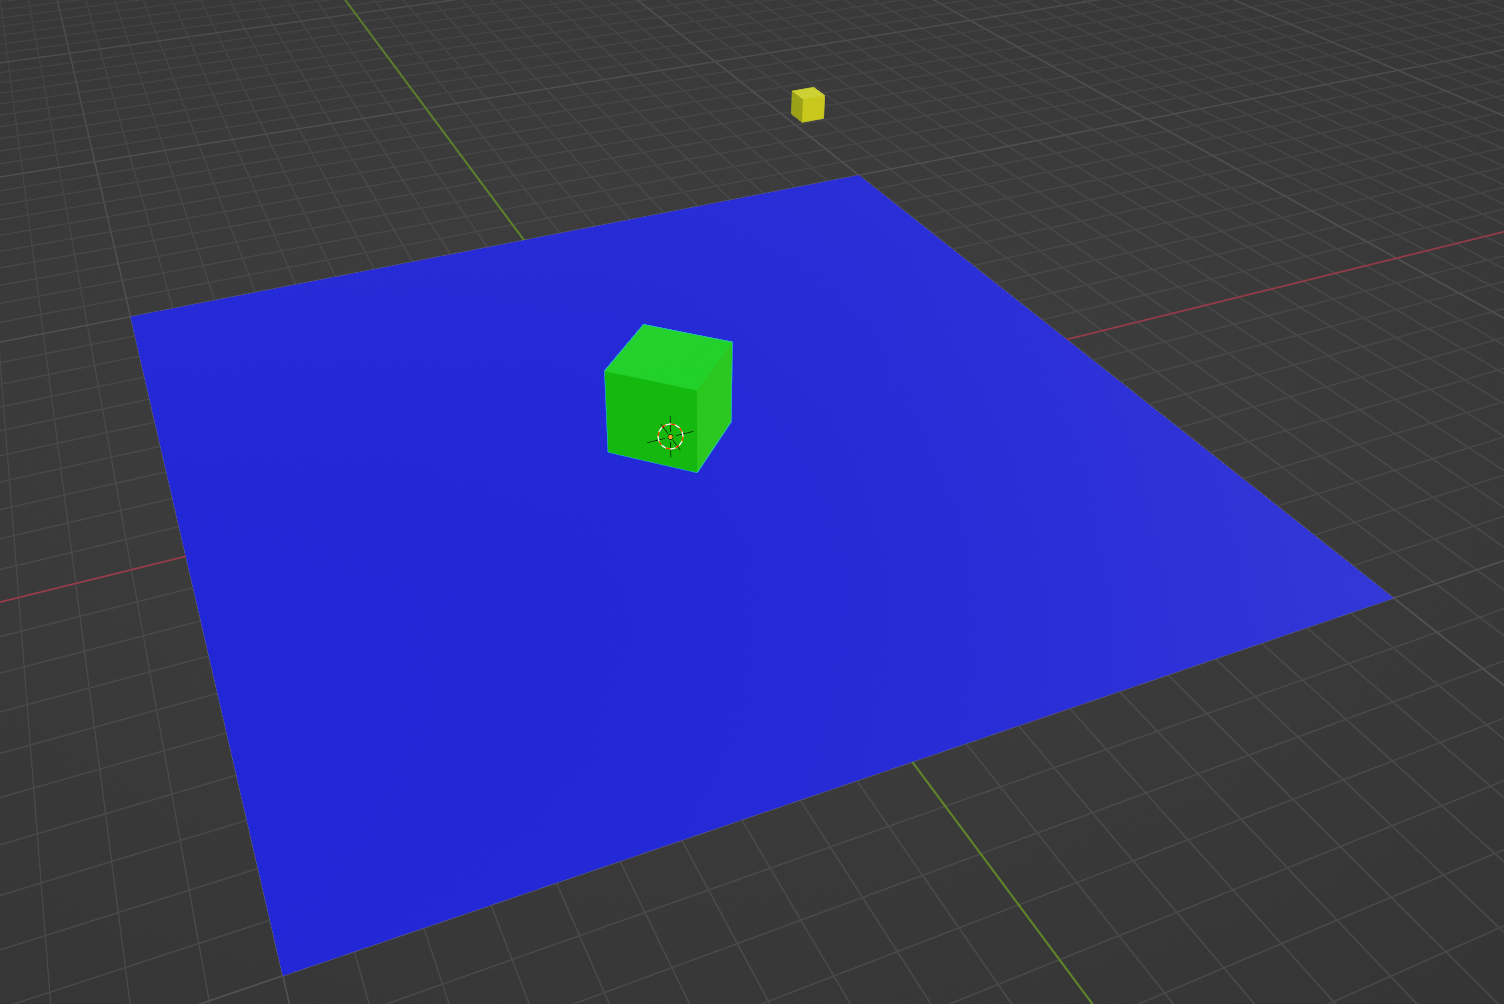
\includegraphics[scale=0.14]{images/SlidesScene/SimpleSceneSeenSetup.png}
\end{figure}

\end{columns}

\end{frame}

\begin{frame}
\frametitle{Scena}
\begin{itemize}
\item Organizziamo gli oggetti da renderizzare in una scena
\item Abbiamo una camera attraverso la quale guardiamo la scena
\item Possiamo mettere uno o più oggetti all'interno della scena
\item Questi oggetti possono condividere un vertex buffer e un pipeline state object
\item Infatti, oggetti diversi possono usare gli stessi vertici e la stessa configurazione della pipeline
\item Ogni oggetto ha un proprio uniform buffer
\end{itemize}
\end{frame}
